\documentclass{svproc}
%
% to typeset URLs, URIs, and DOIs
\usepackage{url}
\def\UrlFont{\rmfamily}
%
% Footnotes:
\usepackage[bottom]{footmisc}
%
% Images:
 \usepackage{graphicx}
%
\makeatletter
\newcommand{\verbatimfont}[1]{\renewcommand{\verbatim@font}{\ttfamily#1}}
\makeatother
%
\begin{document}
\mainmatter  % start of a contribution
\title{Recurring Return on Modeling Investment:\newline A Conceptual Modeling Language and Extensible Compiler}
\titlerunning{Conceptual Modeling Extensible Compiler}  % abbreviated title (for running head)
\toctitle{A Conceptual Modeling Language and Extensible Compiler} % used for the TOC 
\author{Quenio Cesar Machado dos Santos\inst{1} \and Raul Sidnei Wazlawick\inst{2}}
\authorrunning{Quenio C. M. dos Santos et al.} % abbreviated author list (for running head)
\tocauthor{Quenio Cesar Machado dos Santos, Raul Sidnei Wazlawick} % list of authors for the TOC
\institute{Computer Sciences,\\
UFSC - Universidade Federal de Santa Catarina, Brazil,\\
\email{queniodossantos@gmail.com}
\and
Associate Professor of Computer Sciences Department,\\
UFSC - Universidade Federal de Santa Catarina, Brazil,\\
 \email{raul@inf.ufsc.br}}

\maketitle              % typeset the title of the contribution

\begin{abstract}
Proposes a textual programming language that enables conceptual modeling
(similarly to UML classes/associations and OCL constraints) and a compiler
that allows code generation (via extensible textual templates) to any target
language or technology.
Together, the language and the compiler make it feasible
to specify (in a single high-level language) the information of ever-changing,
increasingly distributed software systems. From this single source,
the automated code generation keeps the implementations 
(across the different platforms and technologies) consistent with the specification.
Also, as the technology landscape evolves, these textual models allow the recurring
use of the investment made on their specification.
Unlike other approaches, such as MDA and MPS, the built-in tooling support,
along with the textual nature of this programming language and its extensible templates,
facilitates the integration to the workflow of software developers,
which is expected to promote its adoption. 
A cost-benefit analysis model is also provided, which should assist the stakeholders
in measuring the return of their investment in modeling.
\keywords{conceptual modeling, omg, mda, uml, ocl, mof, mps, mde, mdsd, er, entity-relationship model,
programming language, compiler, code generation, model-driven software development, model-driven engineering, 
modeling investment, classes, associations, constraints, specification, software tools, metaprogramming, 
generative programming}
\end{abstract}

\section{Introduction}
%
In order to address the challenges of the ever-changing, increasingly distributed technologies used on software systems, the Model-Driven Architecture (MDA \cite{mda}) initiative by the Object Management Group (OMG) has been promoting model-driven software development.
In particular, MDA has guided the use of high-level models (created with OMG standards, such as UML \cite{uml}, OCL \cite{ocl} and MOF \cite{mof}) to derive software artifacts and implementations via automated transformations.
As one of its value propositions, the MDA guide \cite{mda} advocates:
\begin{quote}``Automation reduces the time and cost of realizing a design, reduces the time and cost for changes and maintenance and produces results that ensure consistency across all of the derived artifacts. For example, manually producing all of the web service artifacts required to implement a set of processes and services for an organization is difficult and error-prone. Producing execution artifacts from a model is more reliable and faster.''\end{quote} 

The Metaprogramming System (MPS \cite{voelter}) has shown that tooling can assist in integrating high-level, domain-specific models in the development workflow.


\section{Why A New Language?}\label{sec:why}

At this point, one could question: why define a new textual language for conceptual modeling from scratch? Instead of basing it on an standard, richer textual language, such as OWL 2 \cite{owl2}. There are two reasons:
\begin{itemize}
\item\emph{Developer experience}: CML is designed for software developers.
It is intended to enable developers to do \emph{conceptual modeling} much the same way they are used to doing \emph{programming}.
Even the Manchester \cite{owl2manchester} syntax of OWL 2, which was intended to be more user-friendly, does not resemble the syntax of existing programming languages.
Using CML, and its familiar syntax (as we shall demonstrate in the next sections), it is expected that developers will be able to raise the abstraction level of their programs, but still work with a syntax that is familiar to them.
Thus, a new language is necessary to enable the \emph{modeling-as-programming} approach. 
\item\emph{Language evolution}: CML is intended to evolve with the tooling around it.
Unlike the expressive power seen on OWL 2 \cite{owl2} with its breadth of features,
and its ambition to model complete ontologies for the Web,
the CML language and its extensible compiler intentionally support a limited number of features and scenarios.
This initial CML version is expected to be sufficient for the validation of the model-driven development approach taken by CML.
As developers provide feedback, new language features may be added in order to support the extensible compiler and its development scenarios.
\end{itemize}

\section{The Language}\label{sec:lang}
%
\section{The Extensible Compiler}\label{sec:compiler}

In order to realize the CMP \cite{cmp} manifesto's vision,
the CML compiler generates code in any target language based on extensible templates.
A set of core templates is provided by the CML compiler's base libraries.
Third-party libraries can also provide their own templates,
along with their conceptual models,
in order to target specific technologies or platforms.
Developers can also extend existing templates in order to adapt the implementation to characteristics specific to their projects.

Subsection \ref{subsec:overview} will provide an overview of the CML compiler's architecture.
Next, subsection \ref{subsec:templates} will introduce the CML compiler's extensible templates.
Finally, subsection \ref{subsec:modlib} will lay out the CML compiler's mechanism for organizing and sharing conceptual models and extensible templates.

\subsection{Compiler Overview}\label{subsec:overview}

An overview of the CML compiler's architecture is shown in figure \ref{fig:overview}.

\begin{figure}
\centering
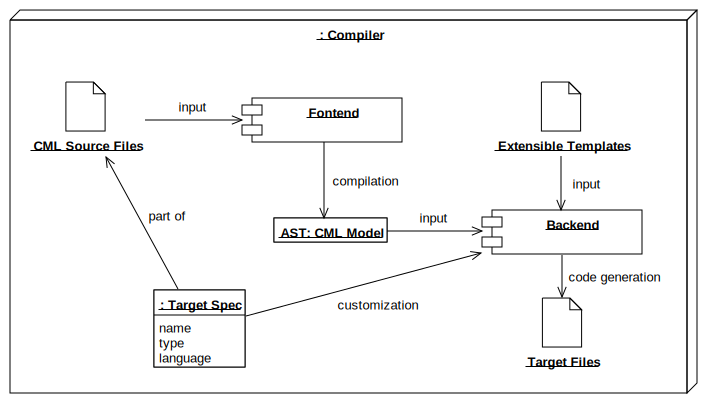
\includegraphics[width=\textwidth]{compiler/figure-overview}
\caption{An architectural overview of the CML compiler.}
\label{fig:overview}
\end{figure}

\subsection{Extensible Templates}\label{subsec:templates}

Terence Parr has formalized and developed the StringTemplate \cite{st} language for code generation. CML extensible templates are implemented in StringTemplate. The CML compiler uses StringTemplate for two purposes:

\begin{itemize}
\item \emph{file names and directory structure:}
each type of target generated by the CML compiler requires a different directory structure.
The CML compiler expects each target type to define a template file named ``files.stg'' (also known as \emph{files template}),
which will contain the path of all files to be generated. The \emph{files template} may use information provided by the \emph{target specification} (introduced in subsection \ref{subsec:overview}) in order to determine the file/directory names. Figure X shows an example of a \emph{files template}.
\item \emph{file content generation:}
each file listed under the \emph{files template} will have a corresponding \emph{content template} that specifies how the file's content must be generated. The \emph{content template} will receive as input one root-level element of the CML model, which will provide information to generate the file's content. The type of model element received as input by the \emph{content template} depends on which function of the \emph{files template} has defined the file to be generated. Figure Y shows a typical \emph{content template}. 
\end{itemize}

For example, ...

\subsection{Modules and Libraries}\label{subsec:modlib}

TODO: Check .NET assembly specification.

TODO: Check Java module specification.

When developing a single application with just a few targets, having a single directory to maintain all the source code is sufficient. But once one needs to develop more than one application (as part of a larger project) and share code among them, it is necessary to separate the common code. Also, some applications cover different domains, and it may be beneficial to separate the code into different CML models.

In order to allow that, CML supports \emph{modules}. Grouping a set of elements of a CML model, a module in CML is conceptually similar to a UML \cite{uml} package. Physically, each module is a directory containing three sub-directories:

\begin{itemize}
\item \emph{source}: where the CML source files reside.
\item \emph{templates}: optional directory containing templates for code generation.
\item \emph{targets}: created by the CML compiler to contain each target sub-directory, which in turn contains the target files generated for a given target.
\end{itemize}

Under the \emph{source} directory, the module will be defined by a \emph{module specification}. If a module needs to reference CML model elements in other modules, then an import statement should define the name of the other modules. The compiler will then compile the imported modules before compiling the current module.

In order for the compiler to find the other modules, they must be in a directory with the module's name in the same directory where the current module is placed.

CML modules have no versions as they are maintained in the same code repository with the other modules they import. However, one can package a module as a library, which will have a version and the same name as the module. This library in turn can be published into a public (or company-wide) \emph{library site} in order to be shared with other developers.

A CML library is just a packaged, read-only module with a version of the format: 

\verbatimfont{\small}
\begin{verbatim}
revision[.accretion][.fix]
\end{verbatim}

TODO: check semantic versioning

Where:
\begin{itemize}
\item \emph{revision} is the number of a library release incompatible with any previous releases with a lower revision number.
\item \emph{accretion} is the number of a library release compatible with any previous accretion number of the same revision.
\item \emph{fix} is the number of a library release that fixes an issue in a previous accretion.
\end{itemize}

Compatible versions do not change or remove public elements of the library's CML model (or function/parameters from the library's templates) but only add new elements. Fixes cannot change the library's public elements; only internal elements. These rules may be enforced by the CML compiler when packaging and publishing new versions of a library.


\section{The Development Workflow}\label{sec:workflow}
%
\section{The Cost-Benefit Analysis Model}\label{sec:cba}
%
\section{Conclusion}\label{sec:conclusion}

The CML language and the compiler make it feasible
to specify (in a single high-level language) the information of ever-changing,
increasingly distributed software systems.
From a single source,
the automated code generation keeps the implementations 
(across the different platforms and technologies) consistent with the specification.
Also, as the technology landscape evolves, these textual models allow the recurring
use of the investment made on their specification.
This first CML version has been designed for the initial validation of the model- driven development approach taken by CML.
As developers provide feedback,
new language features may be iteratively added in order to enable the extensible CML compiler to support new modeling/development scenarios.
\appendix
\section{The Concrete/Abstract Syntax}\label{sec:spec}
%
This appendix provides a formal description of the concrete syntax, along with its mapping to the abstract syntax.
%
\bibliographystyle{spmpsci}
\bibliography{references}
%
\end{document}
